\section{Ethereum}
Ethereum is a blockchain platform for building decentralized applications in which both code and state is stored, publicly on a blockchain.
Each transaction can cause code execution and so update state, emit events and write logs.
In order to interact with this code on the blockchain we can build frontend web interfaces to respond to events and read logs.

Ethereum became the most popular platform for creating:
\begin{itemize}
    \item NFTs: we will see them more in depth in the future;
    \item ICOs (Initial Coin Offering): a company seeking to raise money to create a new app or service on the blockchain, can launch an ICO as a way to raise funds.
    Who wants to participate in this idea can buy new cryptocurrencies token issued by the company, once the project is done the token may have some utility in the project or represent a stake (kind of shares of the company).
\end{itemize}

Moreover the idea of code on the blockchain is not only related to money but also allow:
\begin{itemize}
    \item crowdfunding
    \item tokens
    \item Self Sovereign Identity (SSI)
    \item supply chains
    \item internet of things: tracing sensors data
    \item voting
    \item ...
\end{itemize}
and in Ethereum smart contracts allows:
\begin{itemize}
    \item transparency: all participants in a blockchain run the same code, each verifying the other, so smart contract must be deterministic, also the logic of the contract is visible to all because the code is publicly available on the blockchain.
    To solve the privacy problem zero-knowledge proofs may be used;

    \item more flexibility than bitcoin's scripts: the Ethereum VM is Turing complete but nodes must be rewarded for executing smart contracts so the users have to pay for the execution cost.
\end{itemize}

\subsection{Ethereum VS Bitcoin}
Like Bitcoin Ethereum too is a transaction-based deterministic state machine which uses a virtual machine that executes contracts and operations in order to alter the state.
Anyone can create its own state transition functions but different from Bitcoin, in Ethereum there is no UTXO concept, instead balance tracking is done through accounts, like in a bank.
The global shared state of Ethereum is stored in a multitude of accounts which interact one another through a message-passing paradigm.

Both Ethereum and Bitcoin are public and permissionless blockchains in which addresses are generate by keys, transactions are signed through a digital signatures and block contains data and code.
Ethereum used PoW until September 2022, when they decided to switch to Proof of Stake, also it's native cryptocurrency is Ether (ETH) and it is deployed on top of Kademlia.


\subsection{Accounts}
Each account has an identifier of 20 byte and a state associated with it.
Two types of accounts are available:
\begin{itemize}
    \item \emph{externaly owner} accounts: are controlled by a private keys and have no code associated with them.
    These accounts are the personal one owned by someone, here too having the private key allows access to funds and to contracts invocation.
    In the state associated with the account there are:
    \begin{itemize}
        \item address;
        \item Ether balance;
        \item nonce: the total number of transactions emitted by that account.
    \end{itemize}
    Each account can of course send transactions to transfer Ether or trigger smart contracts.
    In the transaction from an EOA to a EOA there is only written:
    \begin{itemize}
        \item a signature made from the sender's private key;
        \item the address of the receiver;
        \item the amount of wei (fraction of Ether) to transfer.
    \end{itemize}
    
    \item \emph{contract} accounts: have code associated with them and are completely controlled by the associated code.
    In the state associated with the account there are:
    \begin{itemize}
        \item contract code;
        \item persistent storage for contract variables;
        \item Ether balance (that can be sent and received);
        \item nonce: number of messages sent from this account.
    \end{itemize}
    Of course there is no associate private key.
\end{itemize}

\section{Smart Contract}
\emph{A smart contract is a computerized transaction protocol that executes the terms of a contract. The general objectives are to satisfy common contractual conditions (such as payment terms, liens, confidentiality, and even enforcement), minimize exceptions both malicious and accidental, and minimize the need for trusted intermediaries. Related economic goals include lowering fraud loss, arbitrations and enforcements costs, and other transaction costs}, from Nick Szabo in 1994.

Basically a Smart Contract is some code automating the \emph{if this happens then do that} part of the traditional contracts but, since the code is run into a computer, the code behaves deterministically without having linguistic interpretations.
Moreover the idea of deploying the code on top of a blockchain allows us to be free from centralized authority.
The code runs on each node of the network and then the network must reach a consensus on the result of the computation.
It's basically a decentralized state machine.

Code of smart contract cannot change and can only be executed by full nodes.
It must perform deterministic computation because the outcome must be the same for every node in order to reach a consensus.
The execution context of a smart contract contains:
\begin{itemize}
    \item transaction context which are the data taken from the transaction that has activated the contract;
    \item internal storage of the contract;
    \item information from block headers of the blockchain.
\end{itemize}

\subsection{Example of smart contract}
\begin{verbatim}
    pragma solidity ^0.4.7;

    contract Coin{
        address public minter;
        mapping (address => uint) public balances;

        event Sent(address from, address to, uint amount);

        constructor() public {
            minter = msg.sender;
        }

        function mint(address receiver, uint amount) public {
            if (msg.sender != minter) return;
            balances[receiver] += amount;
        }

        function send(address receiver, uint amount) public {
            if (balances[msg.sender] < amount) return;
            balances[msg.sender] -= amount;
            balances[receiver] += amount;
            emit Sent(msg.sender, receiver, amount);
        }
    }
\end{verbatim}

\subsection{Lifecycle}
In order to create a smart contract an EOA has to sent a specific transaction in which specifies:
\begin{itemize}
    \item an empty receiver address, because until the contract is deployed there is no address;
    \item the actual code of the smart contract.
\end{itemize}

To interact with a transaction the EOA calls a method of the smart contract through a transaction, to do that the transaction has to contain:
\begin{itemize}
    \item the address of the transaction;
    \item a data field with the called method and the parameters.
\end{itemize}
In general a smart contract can be triggered both by transactions from EOA or from messages from other smart contracts which can call functions inside a contract by specifying the address of the contract, the parameters to that function and the message may also contain Ether to transfer from one contract to the other.

A contract cannot initiate a transaction by itself but when activated can call other contracts, except itself, in this way it could build complex execution paths.
Moreover a contract, once it receives a message, can make computation, write to internal storage, send messages to another smart contract but also create new contracts.

A contract can in the end be destructed if it executes the \verb|selfdestruct| operation.

\subsection{Nonces}
Ethereum has two types of nonces:
\begin{itemize}
    \item transaction nonce: nonce store in the account which tells us the name of transaction that address has sent, or (in the case of smart contracts) the number of contract-creations made by that account.
    It has been introduced in order to protect against transaction duplication and reply attacks, trying to avoid double spending from the same address;
    \item block nonce: used in proof-of-work like in bitcoin one.
\end{itemize}
NB: a transaction specifies only an amount, a destination address and is signed with the sender private key.
If a malicious user replays this transaction it could drain the sender wallet, however adding the account nonce, associated with the sender account and the transaction nonce which tells us which is the number of current transaction for that address we can prevent this attack because the two nonces would not be synced and tampering the transaction one would break the signature.

\subsection{Halting problem}
Since the ethereum programming language is Turing complete we need to take somehow care of the halting problem: it is not possible to tell, just by looking at the program, whether it will take forever not to execute.
On Ethereum this could lead to  denial of service because the execution of an infinite loop will block the virtual machine forever on that computation, and so all the network.
To solve this problem Ethereum introduced the concept of \emph{gas}: the idea is to pay for contract execution giving payed gas to your smart contract.
This feature makes the DoS attacks much more expensive, make executing a smart contract not free and once the gas is finished the EVM halts the execution of the program.

Each computational step executed by the EVM has a fixed \emph{gas fee} associated with the type of instruction and also storage resources required to perform contract actions have some gas fee.

For those reasons we say that EVM is a quasi-Turing-complete machine because it can potentially run any program, ma in the end only if you paid enough gas.

The gas price in Ether is up to the caller, but of course low price means low priority for your transaction, also the caller can specify a gas limit, which is the maximum gas that the user wants to spend.
Gas is measured in \emph{gwei}, the maximum fees are $fee = gas\_price \cdot gas\_limit$ which is the maximum amount of wei the sender is willing to pay for transaction.
Moreover the gas paid are rewards for miners for the effort to run computations and validate transactions.

Ethereum has also a limit on block gas so miners consider a block full when transaction's gas costs reach limit.

Algorithm if enough gas is found:
\begin{verbatim}
    if gas_limit * gas_price > balance:
        halt

    balance -= gas_limit*gas_price
    gas = gas_limit
    ...
    code deducting from gas the amount required
    to run the code
    ...
    balance += gas
        # return remaining gas to the balance
\end{verbatim}

If instead the gas is not enough, the transaction is considered invalid and:
\begin{itemize}
    \item the transaction aborts;
    \item state of the blockchain reverts to previous state;
    \item $gas\_limit \cdot gas\_price$ is still deducted from balance, because the node has spent the effort to run the calculations before running out of gas.
\end{itemize}

\subsection{Transaction structure}
The transaction is serialized using the recursive length prefix encoding scheme and contains:
\begin{itemize}
    \item TO field: a 20 byte ethereum address that can hold any value.
    If the to field is not valid the Ether sent are burnt.

    \item VALUE and DATA fields: they can be significative or null:
    \begin{itemize}
        \item if only value is significative: the transaction is a payment;
        \item if only data is significative: the transaction is a function invocation;
        \item if both value and data are significative: the transaction is both a payment and an invocation.
    \end{itemize}
    The VALUE field contains the amount transmitted by the transaction:
    \begin{itemize}
        \item if it's a transaction to a EOA is the added balance to the target;
        \item if the destination is a contract:
        \begin{itemize}
            \item if no function is found, then it will increase the balance of the target;
            \item otherwise the function named in the data payload must be \emph{payable}, which means that accept Ether from the caller.
        \end{itemize}
    \end{itemize}
    The DATA field means:
    \begin{itemize}
        \item for transaction to a contracts account: 4 bytes as the \emph{function selector}, it is the first 4 bytes of the Keccak-256 hash of the function's prototype and allows to unambiguously identify which function to invoke, the \emph{function arguments} which are encoded to the rules of the various elementary types;

        \item for contract creation transactions: contains the compiled bytecode which will create the contract.
    \end{itemize}

    \item GAS PRICE;
    \item GAS LIMIT;
    \item V, R, S: signature components of an ECDSA digital signature of the originating EOA, it allow to compute the address of the account sending the transaction.
\end{itemize}

\section{Solidity}
The idea behind web 3.0 is a paradigm shift from web 2.0:
\begin{figure}
    \centering
    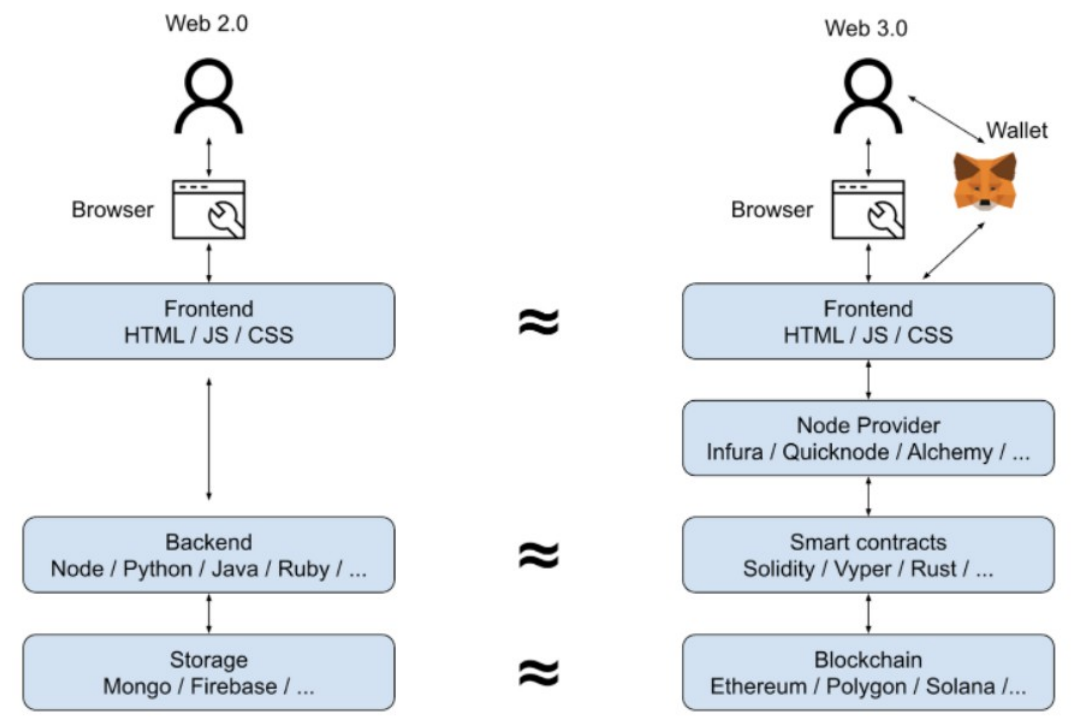
\includegraphics[width=300px]{images/7_Ethereum/01.png}
    \caption{Web 2 and web 3}
\end{figure}
mainly we rely on blockchain to store data and to smart contract to implement functionalities.
Of course we still use the browser as interface to this world, but introducing wallets in the middle to manage secrets and private keys.

In order to communicate with the blockchain we can:
\begin{itemize}
    \item use a third party node as a service provider: (Infura, Alchemy, QuickNode) some node provide an API key that we can use to communicate with the node that than will broadcast our transactions.
    It avoids the setup cost of synchronizing our client to the full blockchain but still relies on third parties, which is a bit in contrast with the idea o blockchain;

    \item running your own client (Geth): but you need to download all the blockchain and then run the services by yourself.
\end{itemize}

Solidity is a contract oriented high level language for the EVM.
It is object-oriented and statically typed language with a syntax very similar to JavaScript in which smart contracts are similar to classes.
Solidity is also used by:
\begin{itemize}
    \item Binance Smart Chain;
    \item Avalanche;
    \item Tendermint;
    \item Hedera.
\end{itemize}

Once the solidity code is written it can be compiled to Ethereum Virtual Machine (EVM) code, then this binary is written on chain through a transaction, it is immutable and lives forever if no destruct function is defined.
While the code is on chain there are no further costs for the deployer, only for the invoker when it invokes function of that contract.

\subsection{Token example}
Let's write a simple smart contract to create tokens on top of Ethereum (those are usually called \emph{layer 2 crypto}) in which only the creator of the contract can mint new tokens and anyone who has an Ethereum account can exchange these tokens.

It is important to understand differences among:
\begin{itemize}
    \item coins: have their own native blockchains, have a specific utility over the whole network, like paying for transaction fees or staking.
    To define a new coin you need to build a new blockchain or fork an existing one to define a new coin;

    \item token: are built on pre-existing blockchains and have a similar role to coins.
    However they are mainly used in their own projects.
    Are simpler to create because they are implemented as smart contract and leverage the security and reputation of an existing blockchain.
\end{itemize}

Our token will be implemented with this contract:
\begin{verbatim}
    pragma solidity >= 0.4.16 < 0.9.0;
    contract Token {
        address public minter;
        mapping (address => uint) balances;

        constructor() public {
            minter = msg.sender;
        }

        function mint(address owner, uint amount) public {
            require (msg.sender = minter);
            balances[owner] += amount;
        }

        function send(address receiver, uint amount) public {
            if (balances[msg.sender] < amount) return;
            balances[msg.sender] -= amount;
            balances[receiver] += amount;
        }

        function queryBalance(address addr)
            public view returns (uint balance) {
                return balances[addr];
            }
    }
\end{verbatim}

\subsection{Pragma directive}
The \emph{version pragma} defines the versions range of the compiler which can be used to compile the specific code.
It is used to reject compilation with future compiler versions that might introduce incompatible changes, which is likely in languages in high evolution.
The \^ is used to pin a version, without it every version after it could be used.

\subsection{Types}
As we can see it the language is statically typed and the type of each variable is specified at compile time, but most types can be cast.
The main types are:
\begin{itemize}
    \item \verb|bool|, \verb|uint8|, \verb|uint16|, ..., \verb|uint256|, \verb|int8|, ..., \verb|int256|;
    \item \verb|address|;
    \item \verb|string|;
    \item \verb|byte[]|;
    \item \verb|mapping(keyType => valueType)|;
\end{itemize}

\subsubsection{address}
An address is a 20 byte value represented in hexadecimal prefixed with 0x.
It does not allow arithmetic operations and is uses to store addresses of accounts (an EOA address is the hash of the public key of the EOA).
Some ways to assign values to an address:
\begin{verbatim}
    address myAddress = 0xE0f5206BBD039e7b0592d8918820024e2a7437b9;
    address emptyAddress = address(0);

        // assign the contract current address
    address current = address(this);
        // assign address of the issuer of the transaction/message
    address sender = msg.sender;
\end{verbatim}

An address has several properties to query:
\begin{itemize}
    \item \verb|address.balance|: the balance in Wei of the address;
    \item \verb|address.code|: the code at the address, which could be empty.
\end{itemize}

\subsubsection{mapping}
A mapping data type appears like a hash table which provide lookup and writes but it is implemented in a different way with respect to other programming languages, because of the memory model adopted by Solidity.
It is important to notice that key data is not stored in the memory, only it's hash is used to look up the value, which is directly stored at the resulting position.
Avoiding a linked list for that bucket operations are $O(1)$.

\subsection{Data store}
In Solidity we can have two types of data store:
\begin{itemize}
    \item storage: variables stored permanently on the blockchain which are stored in the state tree (Patricia Merkle trie) of the block.
    This storage is expensive so it should be limited as much as possible and some gas is refunded when deleted;

    \item memory: is memory used during the function execution and is cleared after the function execution.
    Contains temporary variables, is cheap and should be used whenever possible.
    Data in this memory can be defined using the \verb|memory| keyword.    
\end{itemize}

The storage model of solidity is like a huge array initially filled with 0.
Each value in the array is 32-bytes wide and can contain $2^{256}$ values and each state variable declared in the smart contract will occupy a slot depending on its declaration position and its type (it's size).
Each variable is an offset in this array, moreover since the array is sparsely populated zeros are not stored and an absent key is defined as a mapping to the value zero.

Static data is stored contiguously starting from slot 0 and following:
\begin{verbatim}
    contract example {
        uint256 a;
        uint256[2] b;

        struct exStruct{
            uint256 name;
            uint256 value;
        };

        exStruct c;
        exStruct d[];

        mapping(uint256 => uint 256) e;
    }
\end{verbatim}
in this example we have:
\begin{itemize}
    \item \verb|a| stored at index 0, it occupies only one slot so it fits perfectly;
    \item \verb|b| stored at indexes 1 and 2 because it's large 64 bytes;
    \item \verb|c| stored at indexes 3 and 4 because contains two value of 32 bytes each;
    \item \verb|d| is stored only at index 5 because compile-time allocation is not feasible due to it's unpredictable size, so actual elements are stored starting at a different storage slot that is computed using a Keccak-256 hash of some starting information.
    The slot 5 actually contains the real size of the array, besides other information, and after hashing the index of this slot we get the actual index of the actual values;
    \item \verb|e| takes the index 6 but it's completely empty.
    The values are stored at $Keccak-256(key || index)$, this is done because hashing only the key we would have the same indexes for each mapping, concatenating with the mapping slot instead we get randomized locations.
\end{itemize}

\subsection{Constructor}
The constructor function is invoked only when initially creating the contract and cannot be called afterwards.
It's optional to declare but if declared it must be declared with the constructor keyword from version 0.5.0.
It's mainly used to customize settings or give an initial state.

\subsection{Transaction properties}
There are some predefined variables and functions defined in the global namespace which provide information on the transactions that has invoked a function:
\begin{itemize}
    \item \verb|msg.sender|: sender of the call or the message (gives the address);
    \item \verb|msg.data|: complete calldata (gives bytes);
    \item \verb|msg.value|: value sent in wei (bytes);
    \item \verb|msg.gas|: gas unused after the execution of the transaction.
\end{itemize}

\subsection{Functions}
The syntax to declare a function is:
\begin{verbatim}
    function getLatestPrice(address token) external override view
        returns (int, uint){

        ...
    }
\end{verbatim}

\begin{itemize}
    \item the keyword \verb|function| to declare a function;
    \item the name of the function;
    \item the list of parameters;
    \item the visibility (\verb|external|);
    \item the mutability (\verb|view|);
    \item the return types (\verb|(int, uint)|).
\end{itemize}

In particular the function visibility can be:
\begin{itemize}
    \item \verb|external|: can be triggered by third parties via transaction or from other contracts.
    If a function \verb|f| is external then it must be called with \verb|this.f()|;

    \item \verb|internal|: can be accessed by the current contract and contracts inheriting from it;
    \item \verb|public|: means external and internal, so no restriction on the caller;

    \item \verb|private|: are accessible only from the contract where they are defined and not by derived contracts.
\end{itemize}

NB: any function or data inside a contract is always visible on the public blockchain, the keywords above only affect how and when a function can be called!
Moreover public and external exists because external functions are sometimes more efficient when they receive large arrays of data.

\subsection{Functions mutability}
\begin{itemize}
    \item \verb|view| functions cannot modify states or all other non-view functions;

    \item \verb|pure| functions cannot read or modify the state or call other non-pure functions, they should be evaluable by only its input and \verb|msg.data| values, without any knowledge of the data on the blockchain.
\end{itemize}

\subsection{State variable visibility}
State variable can be declared:
\begin{itemize}
    \item \verb|public|: allows other contracts to read their values;
    \item \verb|internal|: can only be accessed by the contract who defines it and derived contracts;
    \item \verb|private|: can only be accessed by contracts who defines it.
\end{itemize}

\subsection{Error handling}
\subsubsection{require}
The \verb|require| function tests conditions on function arguments or transaction fields ensuring validity of some conditions that cannot be detected until execution time.
It throws an error and stops execution if some condition is not true and is a state reverting function because it undoes all the changes made in the current call.
It of course consume gas up to the point of failure refunding the remaining gas.

\subsubsection{Events logging}
Events are a way for smart contracts written in Solidity to log that something has occurred.
Interested observers can watch for events and react accordingly, for example JavaScript frontend use to do this to notify the user of a DApp that something happened.
In order to use an event you need to:
\begin{itemize}
    \item declare the event with the \verb|event| keyword;
    \item log the event with the \verb|emit| keyword.
\end{itemize}
events can also be parameterized, for example:
\begin{verbatim}
    pragma solidity ^0.4.21;
    contract Counter {
        uint256 public count = 0;

        // declaring event
        event Increment(address who);
        
        function increment() public {
            // logging event
            emit Increment(msg.sender);
            count += 1;
        }
    }
\end{verbatim}
and can be listened from frontend JavaScript with:
\begin{verbatim}
    counter = web3
        .eth
        .contract(abi)
        .at(address);

    counter.Increment((err, result) => {
        if (err) {
            return error(err);
        }
        log("Count was incremented by address:" + result.args.who);
    });
\end{verbatim}

Events can also be indexed in order to be more easily filtered:
\begin{verbatim}
    pragma solidity ^0.4.21;
    contract Multicounter {
        mapping (uint256 => uint256) public counts;
        event Increment(uint256 indexed which, address who);

        function increment(uint256 which) public {
            emit Increment(which, msg.sender);
            counts[which] += 1;
        }
    }
\end{verbatim}
the keyword \verb|indexed| for the first argument of the event tells the contract that events of type \verb|Increment| can be filtered by \verb||


\subsection{Example of DApp: lottery}
The idea is to implement a lottery on the blockchain, so users can bet extracting a number and at the end we extract one number which is the winning one.
The main problem of this application is how to obtain a source of entropy in a deterministic environment.
Some solutions are:
\begin{itemize}
    \item add an external oracle;
    \item take data from the blockchain, for example blockhash, but in this case miners could perform attacks and cheat influencing the game;
    \item Verifiable Random Functions;
    \item RanDAO.
\end{itemize}

\begin{verbatim}
    pragma solidity ^0.8.0;
    contract SimpleLottery {
        uint public constant TICKET_PRICE = 1 gwei;
        address [] public players;
        address payable public winner;
        uint public ticketingCloses;

        // Specify for how long the lottery will run
        constructor (uint duration) {
            ticketingCloses = block.timestamp + duration;
        }
 
        function buy () public payable {
            require(msg.value == TICKET_PRICE);
            require(block.timestamp < ticketingCloses);
            tickets.push(msg.sender);
        }

        function drawWinner () public {
            require(block.timestamp > ticketingCloses + 5 minutes);
            require(winner == address(0));
            bytes32 bhash = blockhash(block.number-1);
            bytes memory bytesArray = new bytes(32);
            for (uint i; i <32; i++) {
                bytesArray[i] = bhash[i];
                bytes32 rand = keccak256(bytesArray);
                winner = payable(tickets[uint(rand) % tickets.length]);
            }
        }
            
        function withdraw () public {
            require(msg.sender == winner);
            winner.transfer(address(this).balance);
        }

        fallback () payable external {
            buy(); 
        }

        function getContractBalance() public returns (uint) {
            return address(this).balance;
        }
    }
\end{verbatim}

Some notes:
\begin{itemize}
    \item \verb|block.timestamp| is the current block timestamp which is the timestamp when the transaction is inserted.
    It returns a UNIX timestamp and can be used to delay actions.
    It could be manipulated by miners.

    \item we set a time delay between the stopping of the ticket purchase period and the drawing of the win because since the source of the entropy is the blockhash we don't want the player to be able to guess the hash of the block that is used as a randomness source.

    \item contracts cannot access ledgers directly because ledgers are maintained by miners only.
    That's because we need to implement a withdraw function which checks for the actual winner address and pays him.

    \item each address has an associated balance in Ether and in order to query it we have to build a function with returns the balance.
    An address that can receive Ether is a \emph{payable address}, similar to payable functions.
    
\end{itemize}

Some other solidity global variables we can use are:
\begin{itemize}
    \item \verb|block.timestamp|;
    \item \verb|block.number|: number of the current block;
    \item \verb|block.gaslimit|;
    \item \verb|block.difficulty|;
    \item \verb|block.coinbase|: current block miner's address;
    \item \verb|tx.gasprice|: the gas price caller is ready to pay for each gas unit;
    \item \verb|tx.origin|: the first caller of the transaction.
\end{itemize}


\subsection{Sending Ether}
There are two ways of sending Ether:
\begin{itemize}
    \item through a transaction generated by an externally owned account;
    \item transferring Ether between smart contracts: this could be dangerous because the contract may be interact with a never seen before contract and so calling a function of which you don't know the behaviour (this could cause reentrancy attack to take place).
\end{itemize}
A simple solution for the second case is to set a limit of the amount of gas that the called contract can use.

There are three functions we can use to transfer funds:
\begin{itemize}
    \item \verb|address.transfer(value)|: throws an error if the transfer fails and propagates the failure to the caller.
    It has a fixed limit of gas for it's execution of 2300 units;

    \item \verb|address.send(value)|: returns false if transfer fails but does not throw exception, so it's management is up to the caller.
    It has a fixed limit of gas for it's execution of 2300 units;

    \item \verb|address.call(value)|: it's a low level function to call contracts.
    It allows to specifically set gas limit, if no gas is specified it may be an entrypoint for a reentrancy attack.
    \begin{verbatim}
        (bool success, ) = address.call{value: 10 ether, gas: 100000}("");
    \end{verbatim}
\end{itemize}

\subsection{Fallback functions}
It's a function with no name and no function keyword which takes no arguments and doesn't return values, it's also only one per contract.
It cannot be called from inside the contract in which it's written and can include arbitrary logic inside.

It's triggered when another contract calls a function in this contract but the called function does not exists.
If the fallback function is also marked as payable a transaction payment is sent to the contract.

It's useful for contracts with a single type of payment because when a user sends money to the contract the fallback one is invoked.

NB: in Solidity versions greater than 0.6 there is also the \verb|receive| method which is invoked when the payload of the transaction is empty but contains Ether, if it's not defined the fallback one is executed.
The signature is:
\begin{verbatim}
    receive() public payable {
        ...
    }
\end{verbatim}

\subsection{Function modifiers}
Solidity also allows to declare custom function modifiers:
\begin{verbatim}
    pragma solidity ^0.6.0;
    contract Token {
        mapping (address => uint) public balances;
        constructor () public {
            balances[msg.sender] = 1000000;
        }

        modifier only_with_at_least (uint x) {
            require(balances[msg.sender] >= x);
            _ ;
        }

        function transfer(uint amount, address dest) 
                public only_with_at_least(100) {

            balances[msg.sender] -= amount;
            balances[dest] += amount;
        }
    }
\end{verbatim}
this pattern is useful to avoid mixing of pre-condition logic and state-transition logic, also allows to reuse the same modifiers in different contexts.

\section{Smart contract security}
DAO which stands for Decentralized Autonomous Organization is a term introduced by Vitalik Butlerin in 2013 to address an organization whose management is decentralized and decisions are automatized through smart contracts.
This way finantial transactions and trading rules encoded in a smart contract and removes the need for a central governing authority, moreover it reduce costs and should provides more control and access to investors.

The idea is to build a platform that allows everyone with a project to pitch their idea to the community for funding, the investors from anywhere in the world can send Ether to a unique wallet in exchange for DAO tokens which give you voting rights.

Once the proposal passes a preliminary's curator check, the various owner's of the DAO tokens can vote it proportionally to their tokens, once a proposal is approved by quorum of all tokens the contract automatically transfer Ether to the smart contract that represent the proposal and the stakeholders receive rewards if the project returns a profit.

\subsection{Reentrancy and The DAO}
The first DAO was created in May 2016 from Slock.it with the idea of connecting smart locks to the blockchain: user of AirBnb submits payment to the Ethereum blockchain and the slock server, which acts as a Ethereum client, receives the transactions.
Once the transaction is received the server unlocks the door and let the customer enter the room.

The slock.it DAO launched the project on 30th April of 2016, which resulted in the largest crowdfunding in history, raising 12M Ether.
During the first weeks security issues were raised and a big community called for a moratorium, however those issues were not addressed fast enough and on 18th June 2016 members of the Ethereum community noticed that funds were drained from the DAO, with full ETH balance drained from the contract.

Let's suppose of having this withdraw function:
\begin{verbatim}
    contract InsecureEtherVault {
        ...
        function deposit() external payable {
            userBalances[msg.sender] += msg.value;
        }
    
        function withdraw() external {
            uint256 balance = userBalances[msg.sender];
            require(balance > 0, "Insufficient balance");
    
            (bool success, ) = msg.sender.call{value : balance}("");
            require(success, "Failed to send Ether");
    
            userBalances[msg.sender] = 0;
        }
        ...
    }
\end{verbatim}
the contract uses the call function to transfer credit which does not specify any gas restriction.

The user can deposit some tokens, then call the withdraw function to be refunded.
If the user calls the function again no refund will be transfered because the balance is zero.

A reentrancy is a scenario in which an attacker performs recursive withdrawals to steal all Ethers locked in a contract.
A procedure is re-entrant if its execution:
\begin{itemize}
    \item can be interrupted in the middle;
    \item initiated over (re-entered);
    \item both runs complete without errors.
\end{itemize}
The attacker can exploit fallback/receive functions of own contract to re-enter the function.

An exploit for the vulnerable contract could be:
\begin{verbatim}
    contract Attack {
        InsecureEtherVault public immutable etherVault;
        ...
        receive() external payable {
            if (address(etherVault).balance >= 1 ether) {
                etherVault.withdraw();
            }
        }

        function attack() external payable {
            require(msg.value == 1 ether, "Require 1 ether to attack");
            etherVault.deposit{value: 1 ether}();
            etherVault.withdraw();
        }
    }
\end{verbatim}
The attacker needs to deploy the contract and call the \verb|attack| function, then:
\begin{itemize}
    \item the contract sends 1 ether to the vulnerable contract;
    \item the deposit function of the target contract is called and the user balance is updated;
    \item the attacker controlled contract calls the \verb|widthdraw| method;
    \item the vuln contract executes the \verb|withdraw| function, then in order to send the fund back it uses the \verb|call| method, without expliciting the gas limit;
    \item the \verb|receive| of the attack contract is executed, which then calls the \verb|withdraw| function again, but the balance is not updated, so there is a new transfer again;
    \item and so on.
\end{itemize}

A general applicable principle to prevent reentrancy: the method is safe if no internal state updates happen after an Ether transfer or an external function call inside a method.

\subsubsection{The hard fork}
A soft fork was proposed first, in order to fix the DAO heist, by blacklisting all the transactions coming from the child DAO of the attacker.
However due to issues in the soft fork the Ethereum community decided for a hard fork: the blockchain come back in the history before the attack transaction.
Due to this fork the Ethereum Classic was born, from the people who didn't want to revert the blockchain.

\subsection{Arithmetic under/overflow}
An arithmetic underflow or overflow arise when an operation requiring fixed-size variable to store a number that is outside the range of the variable's data type:
\begin{verbatim}
    uint8 x = 0;
    uint8 y = x - 1; // y is 255
\end{verbatim}

Let's take the following transfer function as an example:
\begin{verbatim}
    function transfer(address to, uint value) public returns (bool) {
        require(balances[msg.sender] - value >= 0);
        balances[msg.sender] -= balances[msg.sender] - value;
        balances[to] = balances[msg.sender] + _value;
        return true;
    }
\end{verbatim}
the attacker may send a transfer function when his balance is 0, the require guard is satisfied because the number is wrapped becoming a huge number which is greater than 0, then the balance of the user becomes a very large positive number

In order to prevent this kind of vulnerabilities it is advice to use \verb|SafeMath| library.

\subsection{Front running attacks}
Ethereum nodes get transactions and store them in a pool, then take them and form blocks.
All the transactions are visible in the Mempool of a full node for a short before they are executed, so transactions can be observed by nodes to perform an attack.
The miner who solves the block chooses which transactions from the pool, usually ordered by the gas price in order to increase the payout as much as possible.

The idea is to observe a transaction $T$ before it is committed, then produce a transaction $TI$, that pays a higher gas price, this means that miners will execute $TI$ before $T$: the attacker \emph{front run} the user-transaction, taking the profit of knowing the user's transaction.

For example: let's suppose we have a \emph{find this hash} game in which users have to guess the value which hashed is a predefined string.
An attacker can look for the solution in the Mempool, once it's found craft a block with the same answer but with higher gas fee, so hijacking the solution and winning the game.

In order to prevent this attacks contract can implement upper bound on gas price to prevent users from getting preferential transactions ordering (which does not work if the miners are the attackers), or implement a commit-reveal scheme in which transaction is sent with hidden information and after the transaction is included in a block, the user sends another transaction revealing the data that was sent.

\subsection{Transaction ordering attack}
It's basically a race condition attack: if you purchase an item at a price advertised, you expect to pay that price, but if you change the price during the processing of your transaction because someone else has sent a transaction modifying the price before your transaction is complete, then miners can reorder transactions in let you pay the new price.
This happens because the order in which transaction arrives to the mempool is irrelevant, everything that matters is how they are processed, also it is an intrinsic problem with Smart contracts that rely on the state of storage variables to remain at certain value according to the order of transactions.

\subsection{Miners attack}
If a contract relies on block timestamp there could be some issues due to the fact that miners can decide it, in practice it's a bit more difficult because miners cannot choose arbitrary block timestamps cause they must be monotonically increasing and block time set too far will probably be rejected by the network.

It is a good practice to not use timestamps for entropy and avoid time sensitive decisions based on small timestamp differences, it is better to use $block\_number \cdot average\_block\_time$

\subsection{Phishing}
In solidity:
\begin{itemize}
    \item \verb|tx.origin|: is the address of the account that generated the transaction, the original external account that started the transaction;
    \item \verb|msg.sender|: is the immediate account, external or contract account that invoked the function.
\end{itemize}
the \verb|tx.origin| should not be used for authentication because we could trick the user to make a transaction to our contract, which then makes a request to the vulnerable contract, if it checks the user with \verb|tx.origin| we can basically make the user do whatever transaction we want to the vulnerable contract.

\section{Data Layer}
There is no canonical description of the architecture of the Ethereum platform, however we can split it in four layers:
\begin{itemize}
    \item network layer: related to p2p network.
    It uses Kademlia DHT for node discovery, also data exchange and format;

    \item data layer: data structures for accounts, account storage, transactions and receipts, also data serialization.
    Mainly based on Bloom filters and Patricia Merkle Tries, with custom data serialization algorithms;

    \item consensus layer: proof-of-work until september 2022, then proof-of-stake;

    \item application support layer: the ethereum virtual machine.
\end{itemize}

The data structures implemented by exploiting the abstract data types are:
\begin{itemize}
    \item world state trie;
    \item transaction trie;
    \item receipts trie;
    \item storage trie.
\end{itemize}
the serialization formats are:
\begin{itemize}
    \item hex-prefix;
    \item recursive length path (RLP).
\end{itemize}

\subsection{Merkle Patricia Trie in Ethereum}
Merkle Patricia Trie is a data structure created directly for the purpose of Ethereum storage.
As we said before it allows three type of nodes:
\begin{itemize}
    \item branch node: a 17-items node (one element for each nibble and then the value);
    \item extension node: a 2-items node (path, value);
    \item leaf node: a 2-items node (path, value).
\end{itemize}

\subsubsection{Branch node}
Assuming an hex alphabet for the key, then the first 16 items of the node allows for 16 possible branches from 0 to f (hexadecimal characters), when keys, at certain character position starts to differ you store at the $i$-th position child exists if its position corresponds with the next character in one of the keys mapped on the trie.
That position is empty if there s no key with that next character.

The last field instead is a value node: used if the branch node is a terminating node for some keys, while it is a prefix for others.

\subsubsection{Extension node}
It's used to represent a path inside the tree (not suffix), a path common for multiple keys.
This node is used to avoid descending several times following only one path.
It doesn't store any value, only a pointer to the child node that may be a branch node or a leaf node.

\subsubsection{Leaf node}
It's used to terminate a path in the tree, it's basically another compression node different from extension node because it contains the actual value for the key, other than it's representing suffix.

\subsubsection{Merkleizing the patricia trie}
We can make the tree cryptographically secure by pairing each node with its hash.
The root of the node becomes a cryptoraphic fingerprint of the entire data structure and has may be used for look-up in a database and to reference child nodes:

\begin{figure}[H]
    \centering
    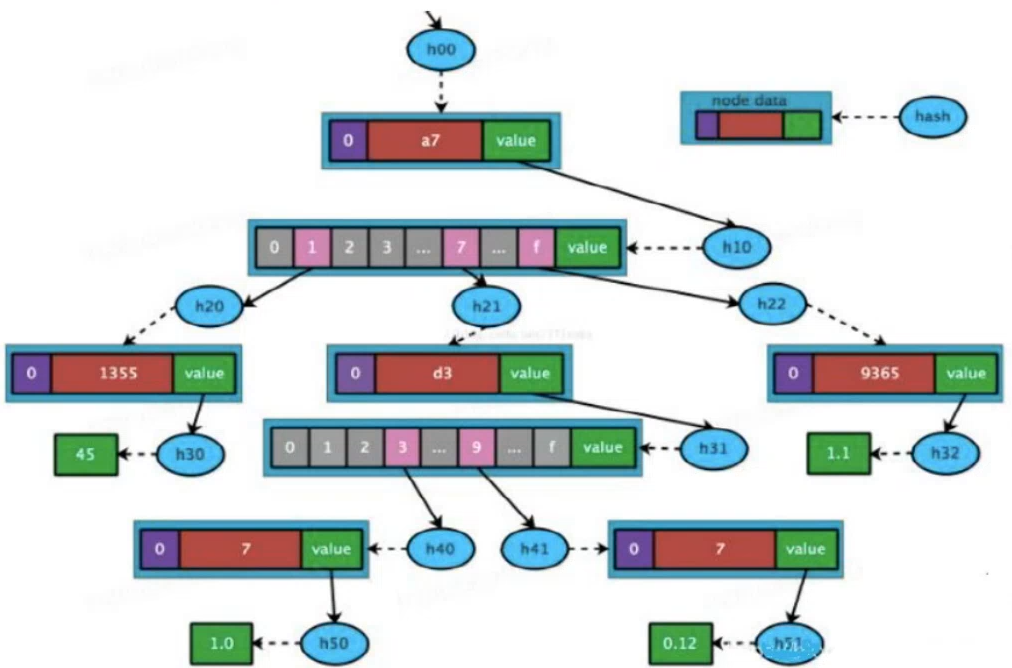
\includegraphics[width=300px]{images/7_Ethereum/02.png}
    \caption{Merkle Patricia Trie in Ethereum}
\end{figure}

\subsubsection{Implementation}
The Ethereum Yellow paper describes the implementation as database based, there is no specified database type but the goal is to store key-value pairs: the hash (kekkak-256 of the content of the node) to the content which produces that hash.
Major Ethereum clients use key-value storage:
\begin{itemize}
    \item Geth uses LevelDB to store recent information which is a key-value store built by Google that can support an ordered mapping from string keys to string values.
    It's a persistent key-value store that can be queried very quickly and is supposed to be run on top of a fast SSD hard disk so that the disk IO is not bottlenecked;

    \item Parity uses RocksDB which is developed and maintained by Facebook Database Engineering Team.
\end{itemize}

\subsection{Serialization}
Values stored in the database are structured data while database only can store strings, also hashing function only takes strings in order to work, so we need some way to serialize those data.
Ethereum uses two techniques:
\begin{itemize}
    \item Hex Prefix Encoding (HP): used for encoding/decoding paths and suffixes in extension and leaf node;
    \item Recursive Length Prefix (RLP): used for encoding and decoding entire nodes.
\end{itemize}

\subsubsection{Hex Prefix Encoding}
Path in extension and leaf nodes are encoded using hexadecimal encoding, so each nibble is mapped to it's hexadecimal representation, a character in the set 0-9, a-f.
In order to save space we compress each couple of nibble into a single byte in order to produce our keybytes.
Then we add as a prefix or tail to the compressed nibbles another byte composed by 2 further nibbles to:
\begin{itemize}
    \item distinguish Leaf and Extension nodes;
    \item convert all paths to a even length (because we can work with bytes, not half byte).
\end{itemize}
The high nibble of the added prefix byte has two bits of information:
\begin{itemize}
    \item lowest-bin encodes oddness of the length of the path;
    \item second-lowest bit encodes the node type
\end{itemize}
basically we have this nibble:
\begin{table}[H]
    \centering
    \begin{tabular}{c|c|c|c}
        Hex & Bits & Node type & Path length \\
        \hline
        0 & 0000 & Extension & even \\
        1 & 0001 & Extension & odd \\
        2 & 0010 & Leaf & even \\
        3 & 0011 & Leaf & odd \\
    \end{tabular}
    \caption{Highest nibble of extension/leaf node encoding}
\end{table}
Then the low nibble of the first byte is zero if the length is even otherwise it is directly the start of the compressed sequence.

So for example the extension node with content \[1,2,3,4,5\] will have lowest bit to 1 because it's length is odd and it's second-lowest bit to 0 because it's an extension node, so nibble 1: 0x112345.
\begin{itemize}
    \item extension \[0,1,2,3,4,5\] will become 0x0001234;
    \item leaf \[0,f,1,c,b,8\] will become 0x200f1cb8;
    \item leaf \[f,1,c,b,8\] will become 0x3f1cb8.
\end{itemize}

\subsubsection{Recursive length prefix encoding}
Afte having serialized each leaf and extension node, we still have trie nodes containing more arrays in every node.
RLP convert a structured value into a single byte array, this way a flatten array can be hashed easily.
RLP is more memory efficient than JSON because it only needs a couple of prefix bytes instead of beginning and ending characters, also JSON it's much more structured allowing both arrays, objects and more.

Won't show all the rules here, a bit useless.

\subsection{MPT in the Ethereum Blockchain}
Ethereum nodes store 3 MPT whose root it stored in the header of the Ethereum block:
\begin{itemize}
    \item World State Trie
    \item Transaction Trie;
    \item Receipts Trie.
\end{itemize}
More information related to Ethereum model like gas, gas price and PoW consensus (now PoS) are store in the block:
\begin{figure}[H]
    \centering
    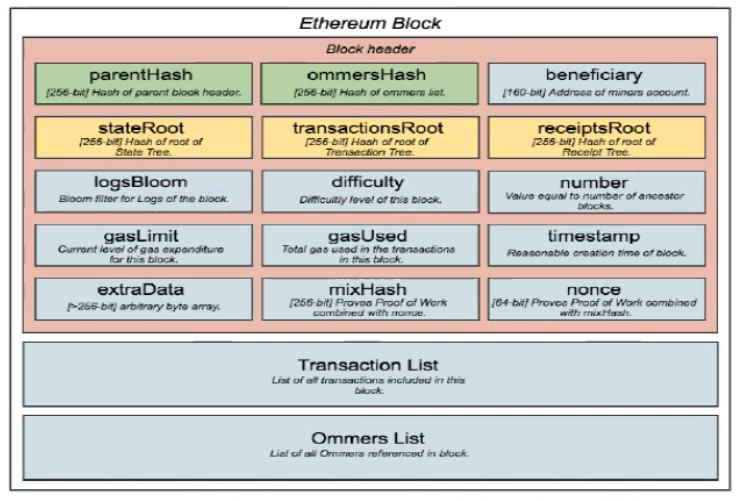
\includegraphics[width=300px]{images/7_Ethereum/03.png}
    \caption{Ethereum block content}
\end{figure}

A complete overview of the block and trie related to the block is:
\begin{figure}[H]
    \centering
    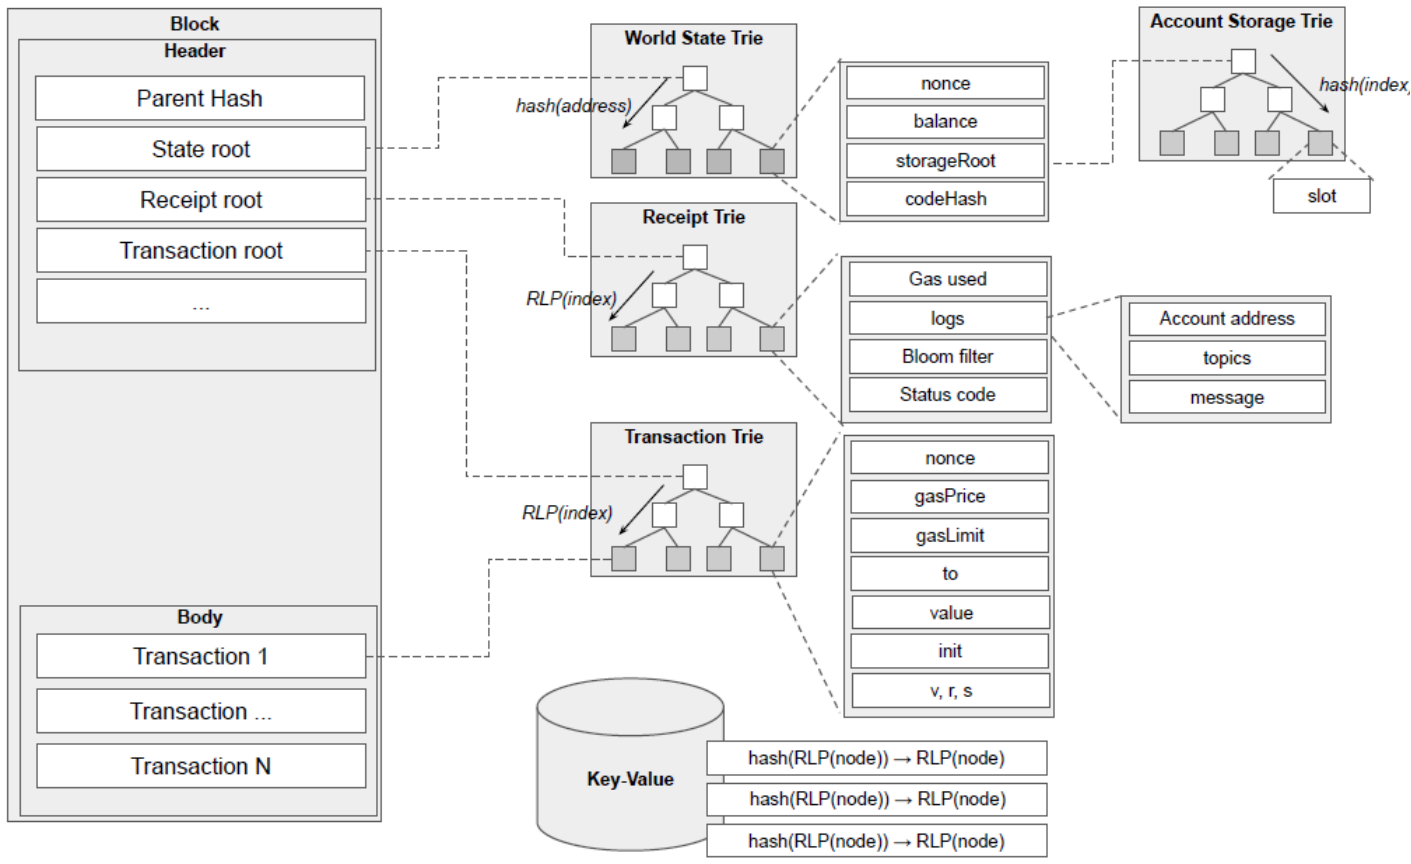
\includegraphics[width=350px]{images/7_Ethereum/04.png}
    \caption{Ethereum block and related Trie}
\end{figure}

\subsection{Transaction MPT}
Transactions are stored in the body of the block, however the transaction trie has one leaf for each transaction in the block.
Each transaction body contains:
\begin{itemize}
    \item nonce: used to avoid reply attack;
    \item gas price;
    \item gas limit;
    \item to;
    \item value;
    \item init: used to initialize smart contract if the transaction is a deploy;
    \item v, r, s: used for signature
\end{itemize}

Since transactions are not executed immediately, because we have to wait for insertion in a block and then synchronize across the network, once a transaction is executed by a node, it creates a record:
\begin{itemize}
    \item in the transaction trie, with al the fields we've seen before;
    \item in the receipt trie.
\end{itemize}
All transactions performed are permanently stored ni the block where they were processed and in the transaction trie, and each transaction is identified by:
\begin{itemize}
    \item an index, which is the path to the leaf;
    \item a value: the transaction itself.
    The value stored in the leaf of the trie is the RLP encoding of the signed transaction
\end{itemize}

\subsection{World State MPT}
Contains a mapping between addresses and accounts.
It's a mutable data-structure, capturing the most recent state of the blockchain, because:
\begin{itemize}
    \item transactions may update the account balance;
    \item transactions may trigger a contract which changes permanent variable in the accounts' storage trie, which implies the update of the \verb|storageRoot|.
\end{itemize}

If the entry is used for a smart contract the \verb|storageRoot| contains the root of the additional MPT structure that contains the global state of the contract memory, while the \verb|codeHash| contains the hash of the code of the contract.
If instead the entry is used for externally owned accounts those fields are empty.

\subsection{Transaction Receipt MPT}
When a transaction is submitted to a blockchain, it is not executed immediately, because of this a user submitting the transaction cannot have its results immediately.
The Ethereum solution says that the result of each transaction execution is stored in a receipt which is stored in the Transaction Receipt MPT.
By analyzing this trie the user that submitted a transaction can observe when the transaction is executed and analyse log messages.
One entry in this trie is created for each transaction, it may contain several information like if the transaction is executed correctly and a set of log generated by the execution of the contract triggered by the transaction.

The receipt then contains the following fields:
\begin{itemize}
    \item a status code of the transaction result, expressed as a number;
    \item cumulative gas used in the respective block after execution of current transaction (the gas consumed by all previous transactions and the recent one);
    \item a list of log entries;
    \item a Bloom filter built hashing the information included in the log entries to speed-up the searching
\end{itemize}

\subsection{Storage MPT}
It's directly modified via a smart contract byte-code using the \verb|STORE| instruction.
Every key in this trie is an index of a slot stored in the leaf node, the key is furthermore hashed.
The index represents one or more global variables in the smart contract.





